\documentclass[compress, smaller, serif, 9pt]{beamer}


\mode<presentation>
{
  \usetheme{Montpellier}
  %\setbeamercovered{transparent}
  % or whatever (possibly just delete it)
}
% or whatever
%\setbeamertemplate{footline}[frame number]
\beamertemplatenavigationsymbolsempty
\beamertemplatetransparentcovereddynamic

\usepackage[english,frenchb]{babel}
\usepackage[utf8]{inputenc}
% or whatever
%\setbeamertemplate{footline}[frame number]
\beamertemplatenavigationsymbolsempty
\beamertemplatetransparentcovereddynamic
\usefoottemplate{%
       \tinycolouredline{blue!03}%
       {
           \hspace{11.5cm}{\color{black!50} {\insertframenumber $/$ \inserttotalframenumber} \hfill}
       }%
}


% Definitions
%\input{def}
% Raccourcis
%\input{raccourci}

% Beamer settings
%\setbeamercolor{structure}{fg=myem!120}
%\setbeamercolor{example}{bg=LightYell,fg=StroYell}

% \setbeamercolor{alerted text}{fg=lightred}
% \setbeamertemplate{blocks}[rounded][shadow=true]
% \newcommand{\exampletext}[1]{{\usebeamercolor[fg]{example text} #1}}
% \newcommand{\structuretext}[1]{{\usebeamercolor[fg]{structure} #1}}
% \usefonttheme[onlymath]{serif}
% \renewcommand{\thefootnote}{\fnsymbol{footnote}}

%\setbeamerfont{sidebar}{5pt}

\usepackage{amssymb}
%\usepackage[T1]{fontenc}
\usepackage{amsmath,amsthm,bm}
\usepackage{pgf}
\usepackage{algorithmicx}
\usepackage{algpseudocode}

\graphicspath{{./Figs/S05/}{./Figs/S04/},{./Figs/S03/}}

\usepackage[normal]{subfigure}
\newcommand{\goodgap}{%
    \hspace{\subfigtopskip}%
    \hspace{\subfigbottomskip}}

% les macros
\newcommand{\exampletext}[1]{{\usebeamercolor[fg]{example text} #1}}
\newcommand{\structuretext}[1]{{\usebeamercolor[fg]{structure} #1}}

\newcommand{\bydef}{\stackrel{{def}}{=}}
\newcommand{\ici}{\tcb{$\blacktriangleright \;$}}
\newcommand{\icir}{\alert{$\blacktriangleright \;$}}
\newcommand{\iciex}{\exampletext{$\blacktriangleright \;$}}
\usepackage{pifont}
\newcommand{\doigt}{\structuretext{\noindent \Pisymbol{pzd}{43}}}
\newcommand{\doigtr}{\alert{\noindent \Pisymbol{pzd}{43}}}
\newcommand{\doigtex}{{\exampletext{\noindent \Pisymbol{pzd}{43}}}}


\setbeamerfont{block title}{size={\normalsize}}





\title[Statistical Learning]{Machine/Statistical Learning}

\subtitle{Lecture 5: Unsupervised classification\\
K-means and Mixture models}


%\author[Florent Chatelain]{Florent Chatelain}
\institute{Filière SICOM, 3A}
%\logo{\includegraphics[width=.2\textwidth]{logoE3}}

\date{}
%

\begin{document}

\maketitle
\section{Unsupervised classification: clustering}
\begin{frame}
  \frametitle{Unsupervised classification}

  \begin{block}{Assumptions}
  \begin{itemize}
     \item $X \in \mathbb{R}^p$, \quad $Y \in \{1,\ldots,K\} \leftarrow$  $K$ classes
     \item Training set $(x_1,\ldots,x_n)$ \alert{ $\leftarrow$ unknown outputs $y_i$}
  \end{itemize}
  \end{block}
    \begin{block}{Example $(p=2)$}
    \vspace{-5mm}
  \begin{center}
     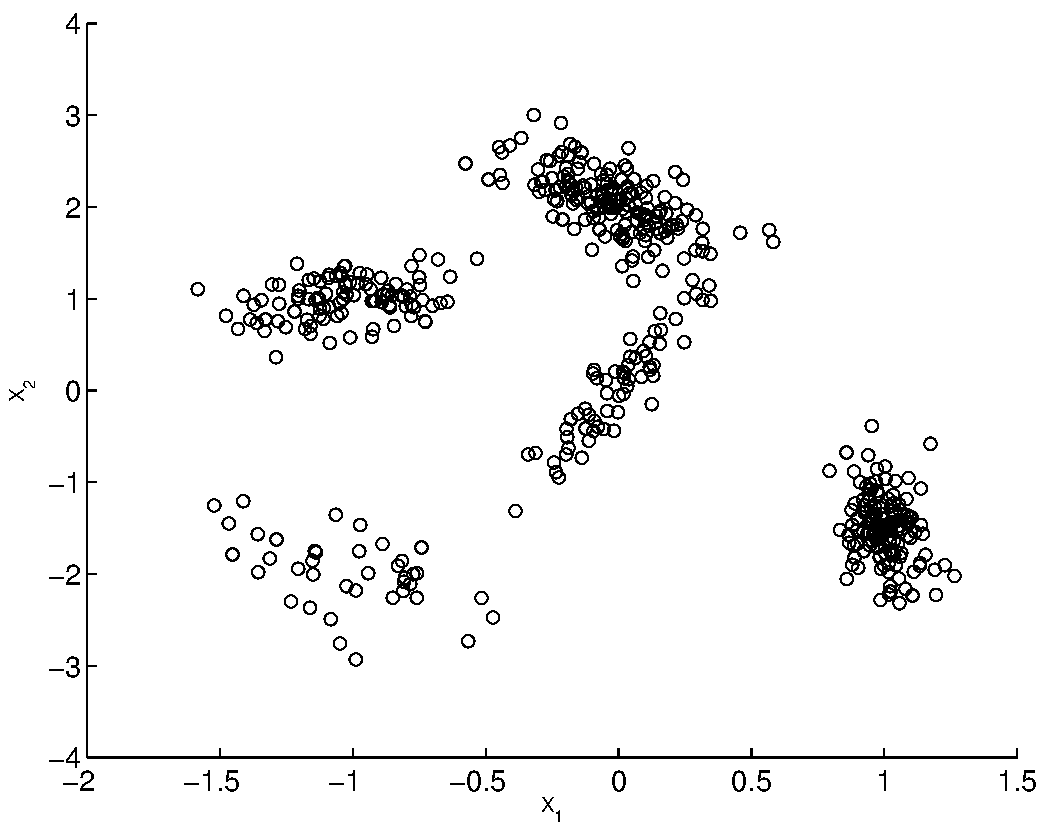
\includegraphics[width=.55\textwidth]{gm_ex_data_us.pdf}%\\
     %\textcolor{blue}
  \end{center}
    \end{block}
\end{frame}

\begin{frame}
  \frametitle{Unsupervised classification: Clustering}
  \begin{block}{Objectives}
  \begin{itemize}
     \item grouping similar data  in the same cluster \structuretext{$\leftarrow$ clustering}
     \item[\doigt] For each  $x_i$, $1\le i \le n$, predict the  class variable $Y_i \in \{1,\ldots,K\}$
  \end{itemize}
  \end{block}
    \begin{block}{Example $(p=2)$}
    \vspace{-5mm}
  \begin{center}
     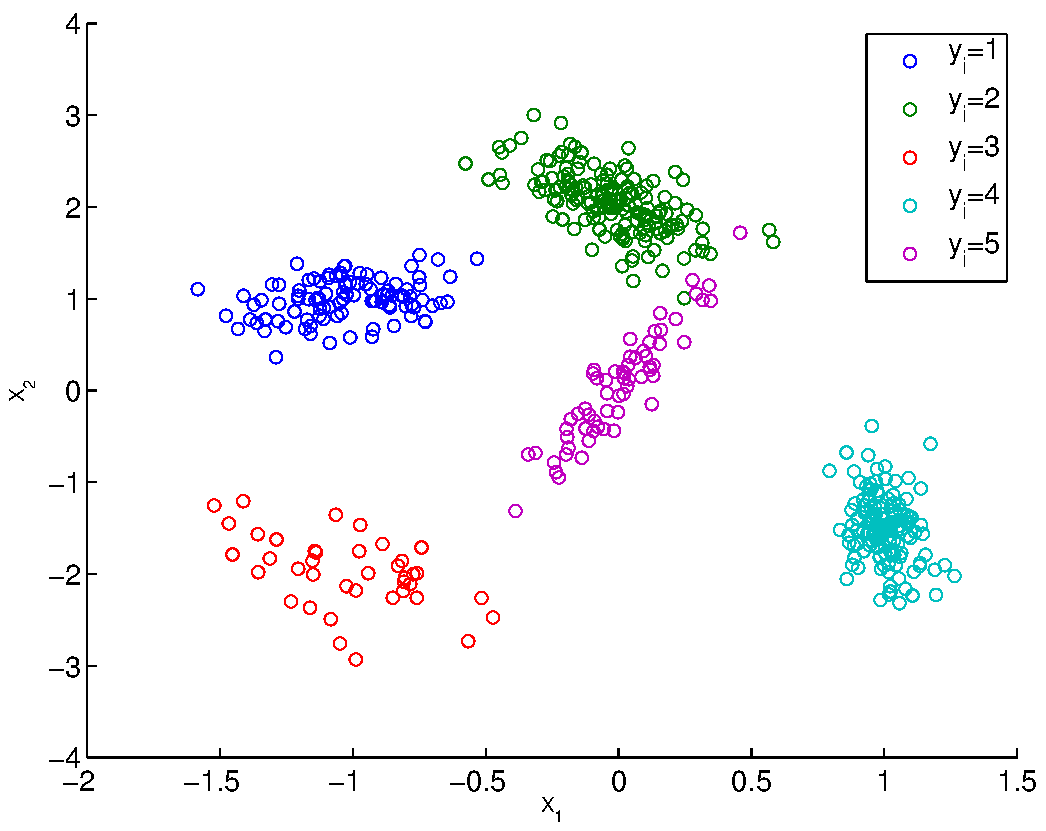
\includegraphics[width=.55\textwidth]{gm_ex_data.pdf} \vspace{-1mm}\\
     \textcolor{blue}{True classes $y_i$  for data $x_i$ ($K=5$)}
  \end{center}
    \end{block}
\end{frame}

\begin{frame}
  \frametitle{Clustering limitations}
  \begin{block}{Combinatorics problem}
  \begin{itemize}
     \item Number of partitions into $K$ classes for a  sized $n$ dataset: {\em Stirling number} of the 2nd kind $S(n,K)$
     \item Number of partitions for a  sized $n$ dataset: {\em Bell number} $B_n= \sum_{k=1}^n S(n,k)$
   \end{itemize}
   {\small
  \begin{tabular}{l|ccccc}
  dataset size $n$ & 2 & 5 & 10 & 100 & 200 \\
  \hline
  $S(n,2)$ ($K=2$ classes) & $1$ & $15$ & $511$ & $6.3\times 10^{29}$ & $8.0\times 10^{59}$ \\
  $S(n,4)$ ($K=4$ classes) & $0$ & $10$ & $34105$ &  $6.7 \times 10^{58}$ & $1.1 \times 10^{119}$ \\
  %\hline
  $B_n$ & $2$ & $52$ & $115975$ & $4.8 \times 10^{115}$ & $6.2 \times 10^{275}$\\
  \hline
\end{tabular}
}

      \begin{itemize}
     \item Remember $\simeq 10^{80}$ atoms in the Universe...
     \item[Pb:]  Exhaustive search (brute-force) not possible in practice
      \item[\doigtr] \alert{local search} around initial  solutions/values $\rightarrow$ sub-optimal
  \end{itemize}
  \end{block}

  \begin{block}{Estimation problem and model selection}
      \begin{itemize}
     \item possible parameters are unknown $\leftarrow$ estimation
     \item Number of classes $K$ possibly unknown $\leftarrow$ model selection
     \end{itemize}
   \end{block}
\end{frame}

\section{Mixture model}

\begin{frame}
   \frametitle{Mixture of distributions}
   \begin{itemize}
      \item Data $X_1,\ldots,X_n$ assumed to be i.i.d. with pdf $f$
      \item $f$ is modeled as a  {\em mixture of distributions}
      \begin{align*}
	f(x)&= \sum_{k=1}^K \pi_k \phi\left( x ; \theta_k \right)
      \end{align*}
      \item $\pi_1, \ldots, \pi_k$ are the relative sizes ($\sum_{k=1}^K \pi_k = 1$) of the classes:
       \begin{align*}
	\Pr\left(Y_i=k\right) &=  \pi_k
      \end{align*}
      \item density $\phi$ is the parametric shape of a class,
      \item parameters $\theta_1,\ldots,\theta_K$ are the {\em centroids}
      of the classes/clusters
 \end{itemize}
   \begin{block}{Latent variable}
   $Y \in\{1,\ldots,K\}$ indicating the class of the r.v. $X$
      \begin{itemize}
      \item $
   Y \sim \textrm{discrete distribution s.t. }   \Pr\left(Y_i=k\right) =  \pi_k, \quad k=1,\ldots,K
       $
        \item $
       X|Y=k \sim \textrm{distribution with pdf }  \phi\left( \cdot | \theta_k \right)
      $
      \end{itemize}
    \end{block}
\end{frame}


\begin{frame}
   \frametitle{Gaussian mixture model}
   \begin{itemize}

      \item Class centroid: $\theta=(\mu \leftarrow \textrm{mean}, \Sigma \leftarrow$   covariance matrix$)$
      \item Density $\phi$ of a class: multivariate normal distribution $\mathcal{N}(\mu,\Sigma)$ pdf
      \begin{align*}
	\phi(x ;\mu,\Sigma) &= \left( \det{(2 \pi \Sigma )}\right)^{-1/2}
	\exp{\left( -\frac{1}{2}(x-\mu)^T \Sigma^{-1} (x-\mu) \right) }
      \end{align*}
      \item Mixture density $\quad f(x)= \sum_{k=1}^K \pi_k \phi\left( x ; \mu_k,\Sigma_k \right)$
 \end{itemize}
 \begin{block}{Example ($p=2$, $K=5$)}
 \end{block}

 \begin{minipage}{.49\textwidth}
 \begin{center}
    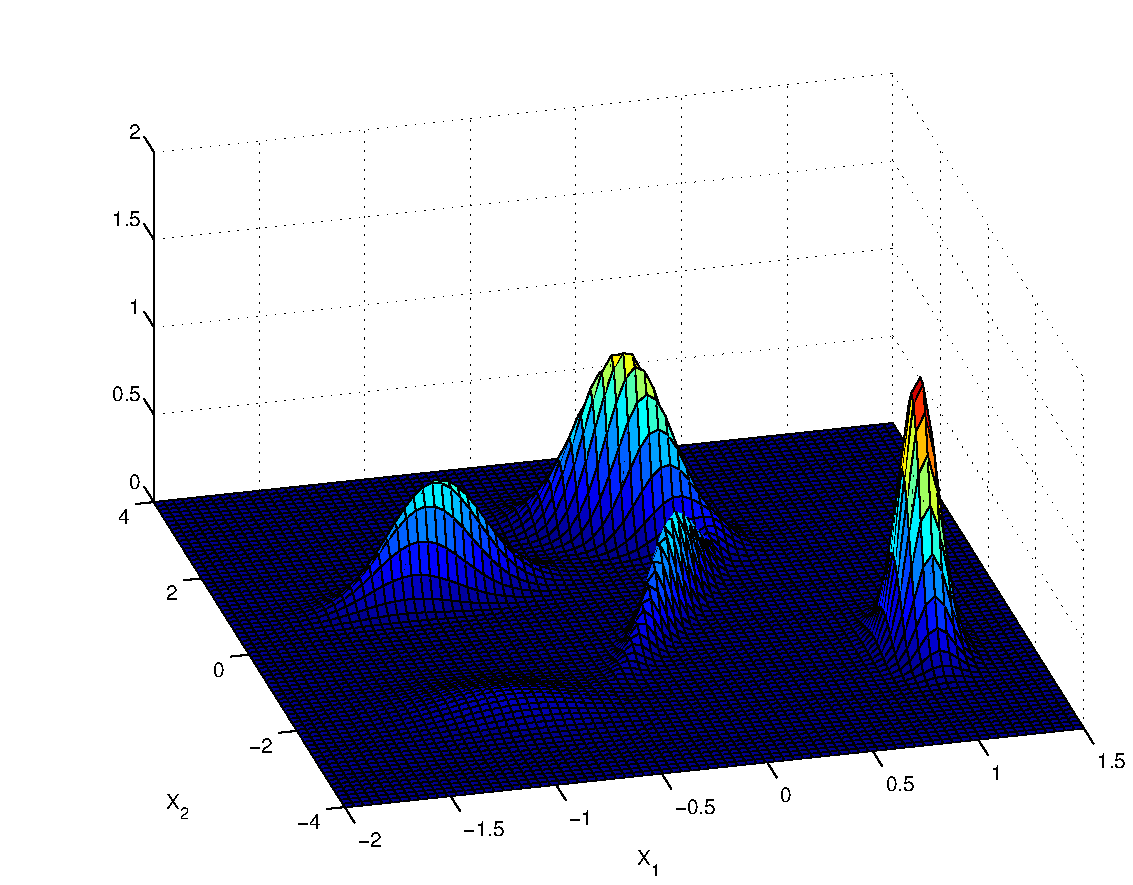
\includegraphics[width=.9\textwidth]{gm_ex_data_pdf.pdf}\\
    \textcolor{blue}{Mixture density $f$}
 \end{center}
 \end{minipage} \hfill
 \begin{minipage}{.49\textwidth}
 \begin{center}
    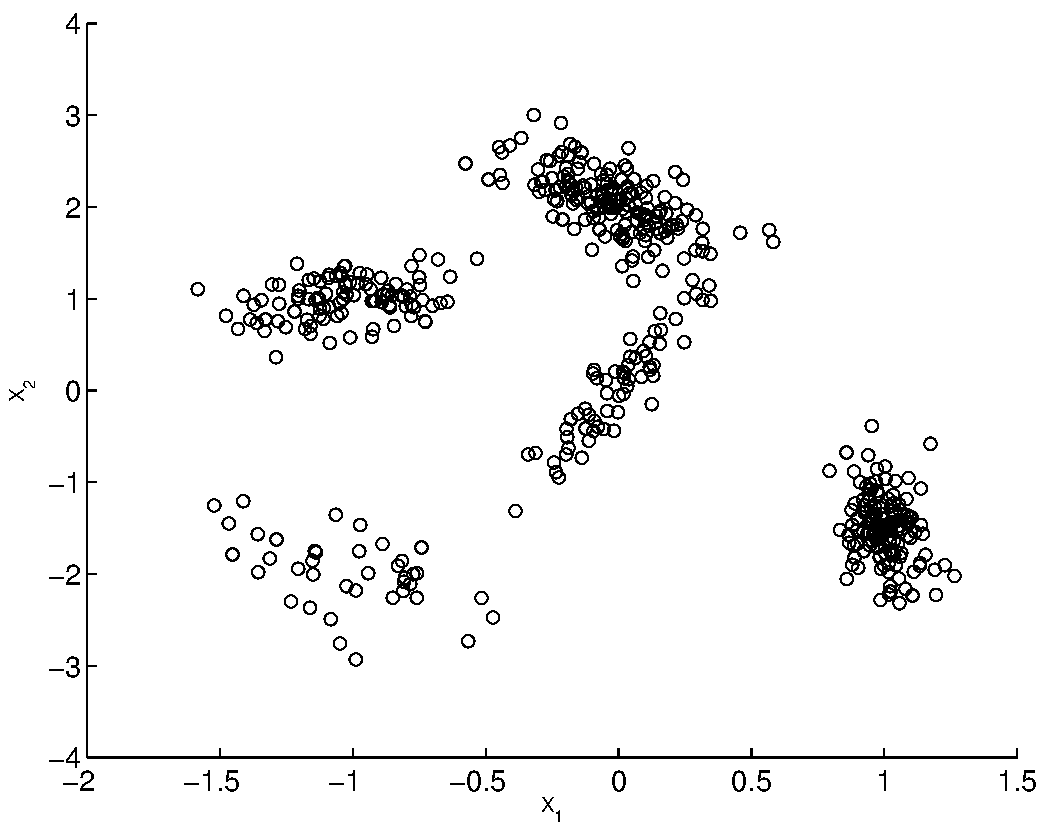
\includegraphics[width=.9\textwidth]{gm_ex_data_us.pdf}\\
    \textcolor{blue}{$n=500$ realizations}
 \end{center}
 \end{minipage}
\end{frame}

\section{Cost based clustering: $K$-means}

\begin{frame}{Cost based approximation: $K$-means}

\begin{itemize}
 \item[Pb:] no simple expression of the Gaussian mixture parameter estimators
 \item[\doigt] several approximations can be conducted to obtain a simple {\em deterministic} cost criterion
\end{itemize}

\begin{block}{First approximation: euclidean distance}
Replace the Mahalanobis distance in the Gaussian density by the simpler euclidean one
$$
(x-\mu_k)^T \Sigma^{-1}_k (x-\mu_k) \rightarrow \|  x-\mu_k \|^2,  \quad \left( \textrm{i.e. }  \structuretext{\Sigma_k= I_p} \right),
$$
\begin{itemize}
 \item[\doigt] cluster centroid for the $k$th class reduces to \structuretext{$\theta_k=\mu_k$} $\leftarrow$ mean vector 
\end{itemize}

 
\end{block}

\end{frame}


\begin{frame}{Cost based approximation: $K$-means (Cont'd)}

\begin{itemize}
 \item[Pb:] no straightforward expression of the Gaussian mixture parameter estimators
 \item[\doigt] several approximations can be conducted to obtain a simple {\em deterministic} cost criterion
\end{itemize}

\begin{block}{Second approximation: hard thresholding}
Binarize the posterior probabilities: for each data point $x_i$,
$$
t_{i,k}\equiv \Pr{\left(Y_i=k |x_i,\theta\right)} = 
\begin{cases}
 1 & \textrm{if } k= \arg \min_{1\le j \le k} \| x_i - \mu_k\|,\\
 0 & \textrm{otherwise.}
\end{cases}
$$
\begin{itemize}
 \item[Csq:] $x_i$ belongs with certainty to the class whose centroid is the closest
 \item[\doigt] \structuretext{hard thresholding} clustering
 \item[\doigt] \structuretext{deterministic} model
\end{itemize}

 
\end{block}

\end{frame}


\begin{frame}{Cost criterion: $K$-means clustering}

\begin{block}{Notations}
 For a given clustering $Y$, let 
 \begin{itemize}
  \item $n_k = \#\left\{ i\ | \ Y_i=k  \right\}$ is the size of the $k$th cluster,
  \item $\widehat{\mu}_k= \frac{1}{n_k} \sum_{i|Y_i=k} x_i$ is the sample mean of the points assigned in the $k$th cluster
 \end{itemize}
\end{block}



Under the previous approximations, maximizing the resulting ``log-likelihood'' reduces to the following 
optimization problem: 
\begin{block}{K-means cost criterion} \vspace{-3mm}
\begin{align*}
\textrm{Minimize} \quad  \structuretext{J(Y)} &= \sum_{k=1}^K \sum_{i=1}^n t_{i,k} \| x_i-\widehat{\mu}_k \|^2,\\
 &= \structuretext{ \sum_{k=1}^K \, \sum_{i|Y_i=k}  \| x_i-\widehat{\mu}_k \|^2},
\end{align*}


\begin{itemize}
 \item[\doigt] $J(Y)$ is the sum of \structuretext{within-cluster} dispersions
\end{itemize}
\end{block}
\end{frame}


% \begin{frame}{Equivalent cost criterion}
% $K$-means cost criterion can be expressed in an equivalent way as:
% \begin{block}{Equivalent expression sum of within-cluster dispersions}
% $$
% J(Y)= \frac{1}{2} \sum_{k=1}^K \, \sum_{i|Y_i=k} \sum_{j|Y_j=k}   \| x_i-x_j \|^2 + \textrm{constant},
% $$
% Proof: replace $\widehat{\mu}_k$ by its expression in the previous, then rearrange the terms
% \end{block}
% 
% 
% \begin{itemize}
%  \item[\doigt] $J(Y)$ is the sum of \structuretext{within-cluster} dispersions
% \end{itemize}
% \end{block}
% \end{frame}


\begin{frame}{Equivalent cost criterion}
%$K$-means cost criterion can be expressed in an equivalent way as:
\begin{block}{(negative) Sum of between-cluster dispersions}
$$
J(Y)= - \sum_{k=1}^K \,  n_k \| \widehat{\mu}_k- m \|^2 + \textrm{constant},
$$
where $m=\frac{1}{n} \sum_{i=1}^n x_i$ is the total mean.
\begin{itemize}
 \item[\doigt] Minimizing the within-cluster dispersion $\Leftrightarrow$ Maximizing the  between-cluster dispersion
 \item[\doigt] General property of clustering algorithms
\end{itemize}
\end{block}
\medskip

\structuretext{Proof:} let $S_T= \sum_{j=1}^n (x_j-m)^T(x_j-m)= \sum_{k=1}^K   \sum_{i|Y_i=k} \| x_i- m \|^2$ be the total dispersion.
\begin{itemize}
 \item Replace $x_i$ by $x_i-\widehat{\mu}_k + \widehat{\mu}_k$, and expand $S_T$
 \item Show that $S_T= J(Y) +  \sum_{k=1}^K \,  n_k \| \widehat{\mu}_k- m \|^2$ (i.e. the cross product equals zero), and conclude by noting that 
  $S_T$ does not depend on $Y$
 %\item Note finally that $S_T$ does not depend on $Y$ 
\end{itemize}
\end{frame}



\begin{frame}{$K$-means: cost criterion optimization}
\medskip

% 
% $\begin{displaystyle}
% \begin{array}{lll}
% \textrm{Note that } & J(Y)&= \sum_{k=1}^K \, \sum_{i|Y_i=k}  \| x_i-\widehat{\mu}_k \|^2,\\
% & &= \min_{\mu_1,\ldots,\mu_K} \sum_{k=1}^K \, \sum_{i|Y_i=k}  \| x_i-\mu_k \|^2,
% \end{array}
% \end{displaystyle}
% $

\setbeamertemplate{blocks}[rounded][shadow=true]


%$K$-means cost criterion can be expressed in an equivalent way as:
\begin{block}{Enlarged optimization problem}
\vspace{-2mm}
$$
\min_{Y,\structuretext{\mu}} J(Y,\structuretext{\mu})= \sum_{k=1}^K \, \sum_{i|Y_i=k}  \underbrace{\| x_i-\structuretext{\mu_k} \|^2}_{J_k},
$$ \vspace{-4mm}
\begin{itemize}
 \item $J_K$ is the quadratic error for the $k$th cluster
\end{itemize}
\end{block}

\setbeamertemplate{blocks}[rounded][shadow=false]
\begin{block}{Remarks}
\begin{itemize} 
\item For a given $Y$, $\min_{\mu} J(Y,\mu)= J(Y,\widehat{\mu}) \equiv J(Y)$  
\item For a given $\mu$, exchanging $Y_i=k$ with $Y_i^{\star}=l$ changes the two quadratic errors
$$\left[ 
\begin{array}{ll}
J_k^{\star} &= J_k - \| x_i - \mu_k \|^2,\\
J_l^{\star} &= J_l + \| x_i - \mu_l \|^2,,
\end{array}\right.$$
Thus $J(Y,\mu)$ is decreased if 
$$ 
\begin{array}{lll}
&  J_l^{\star} -  J_l &\le J_k - J_k^{\star}\\
\Leftrightarrow & \| x_i - \mu_l \|^2 & \le \| x_i - \mu_k \|^2,\\
\Leftrightarrow & x_i \textrm{ is closer } & \textrm{(euclidean distance) from the class $l$ center},
\end{array}$$
\end{itemize}
\end{block}

\end{frame}



\begin{frame}{$K$-means algorithm}


\setbeamertemplate{blocks}[rounded][shadow=true]

\begin{block}{}%{$K$-means algorithm}
{\small
\begin{itemize}
 \item {\textbf{Require:}} $K$ the number of clusters,\\
 \item {\textbf{Initialization:}} 
 Set the centroid $\mu_k$, $1\le k\le K$, to a starting value $\mu_k^{(0)}$,\\
 \item \textbf{For} $t=  1 \to \ldots$ \textbf{until convergence} $\Big($i.e. $\mu_k^{(t)}=\mu_k^{(t-1)}\Big)$ 
 \begin{enumerate}
  \item \structuretext{\textbf{Assignment step:}} assign $x_i$ to the class of the closest center
$$
Y_i^{(t)}=\arg \min_{k=1,\ldots,K} \left\| x_i - \mu_{k}^{(t-1)} \right\|^2, \quad \textrm{for } i=1,\ldots,n
$$
 \item \structuretext{\textbf{Update step:}} update the centroids $\mu_k$, for $k=1,\ldots,K$
 \vspace{-1mm}
 \begin{align*}
  \mu_k^{(t)}&= \arg \min_{\mu_k}  \sum_{i|Y_i^{(t)}=k} \| x_i- \mu_k \|^2= 
  \frac{1}{n_k^{(t)}} \sum_{i|Y_i^{(t)}=k} x_i,% \quad \leftarrow \textrm{cluster sample mean}
 \end{align*}\vspace{-3mm}\\
 i.e. $\mu_k^{(t)}$ is the sample mean of the $k$th cluster
 %where $n_k^{(t)}=\#\left\{i \ | \ Y_i^{(t)}=k \right\}$, and $\mu_k^{(t)}$ is the sample mean of the $k$th cluster
 \end{enumerate}
\end{itemize}



% 
% \begin{algorithmic}
% \Require $K$ 
% \Comment{number of clusters}
% \medskip
% % % %\State $N$ fixé \Comment{Choix de la longueur du filtre adaptatif RLS}
% \State Initialize  
% %\boldsymbol{w_0}$ fixe, pex $\boldsymbol{w_0}= \boldsymbol{0}$
% % \Comment{Initialisation}
% % \State $\bK_0$ fixe, pex $\bK_0= \delta^2 I_{N+1}$, avec  $\delta^2$ grand
% % \Comment{Initialisation}\medskip
% \For {$t=  1 \to \ldots$ until convergence $\big($i.e. $\mu_k^{(t)}=\mu_k^{(t-1)}\big)$ } 
% % \State \textbf{Entrees~:} $X[J]$, $\bY[J]$
% \State Assignment/prediction step: for $i=1,\ldots,n$, assign $x_i$ to the class of the closest center
% $$
% Y_i^{(t)}=\arg \min_{k=1,\ldots,K} \| x_i - \mu_{k}^{(t-1)} \|^2
% $$
% % \Comment{les observations à la date $J$}
% % \State  $e[J] \gets X[J] - \boldsymbol{w_{J-1}}^T \bY[J]$
% % \Comment{Erreur de prediction $\leftarrow  O(N)$ operations}
% % \State  $\boldsymbol{\gamma}_{J} \gets \frac{\bK_{J-1}\bY[J] }{ 1 + \bY[J] ^T K_{J-1} \bY[J] }$
% % \Comment{Maj du Gain de Kalman $\leftarrow O(N^2)$ operations}
% % \State  $\bK_{J} \gets \bK_{J-1} - \boldsymbol{\gamma}_{J} \bY[J]^T \bK_{J-1}$
% % \Comment{Maj de la matrice de precision $\leftarrow O(N^2)$}
% % \State  $\boldsymbol{w_{J}} \gets \boldsymbol{ w_{J-1} } + \boldsymbol{\gamma}_{J} e[J]$
% % \Comment{Correction du filtre  $\leftarrow O(N)$ operations}
% % \State  $\widehat{S}[J] \gets \boldsymbol{w_{J}}^T$ $\bY[J]$
% % \Comment{Calcul de l'estimee à la date J $\leftarrow O(N)$ operations}
% %\EndFor
% \end{algorithmic}
}
\end{block}

\end{frame}

\begin{frame}{Convergence of $K$-means algorithm}

\begin{block}{Convergence}
\begin{itemize}
 \item each step decreases the criterion, 
 \item there is a (huge) finite number of partitions,
 \item[\doigt] the algorithm \structuretext{converges} to a solution (in a finite number of steps)
 \item[\alert{But}] {no guaranty of the solution optimality} (depend on the initialization)...
\end{itemize}
\end{block}

\begin{block}{Stopping criterion}
$K$-means usually very fast for a small/moderate number of clusters $K$, but
\begin{itemize}
 \item running time increases with the number of clusters $K$
 \item in the worst case, can be very slow to converge even for $K=2$,
\end{itemize}
Thus, to shorten the computational time, the algorithm can be stopped when the 
cost criterion does not decrease significantly
\end{block}

\end{frame}


\begin{frame}{Variants/Improvements of $K$-means algorithm}

\begin{block}{Initialization heuristics}
\begin{itemize}
 \item Forgy method
\begin{itemize}
 \item pick randomly $K$ observations  from the dataset as initial centers,
 \item run $K$-means algorithm with these starting values
 \item repeat these 2 steps several times and retain the best (cost sense) clustering 
\end{itemize}
 
\item lot of variants: \texttt{Random partitions}, \texttt{k-means++}, \texttt{power init.}
\item[\doigt] may lower the computation time of one run,
\item[\doigt] can give some guaranties that the  solution is competitive w.r.t. to the optimal one.

\end{itemize}

\end{block}


\begin{block}{Choice of the distance}

\begin{itemize}
 \item Standard $K$-means based on the squared $\ell_2$ (euclidean) distance.
 \item Other distance can be considered: e.g. using $\ell_1$ distance yields
 the $K$-medians algorithm where the cluster centroid becomes the median
 %$\leftarrow$ may be more robust to possible outliers in a cluster\\
 ({\em Exercice: show this}, cf 2015-16 exam statement)
\end{itemize}
\end{block}

\end{frame}



\begin{frame}
   \frametitle{K-means initilization}
   \begin{block}{Sensitivity to initialization/data geometry/number of classes}
   \end{block}
   \begin{center}
    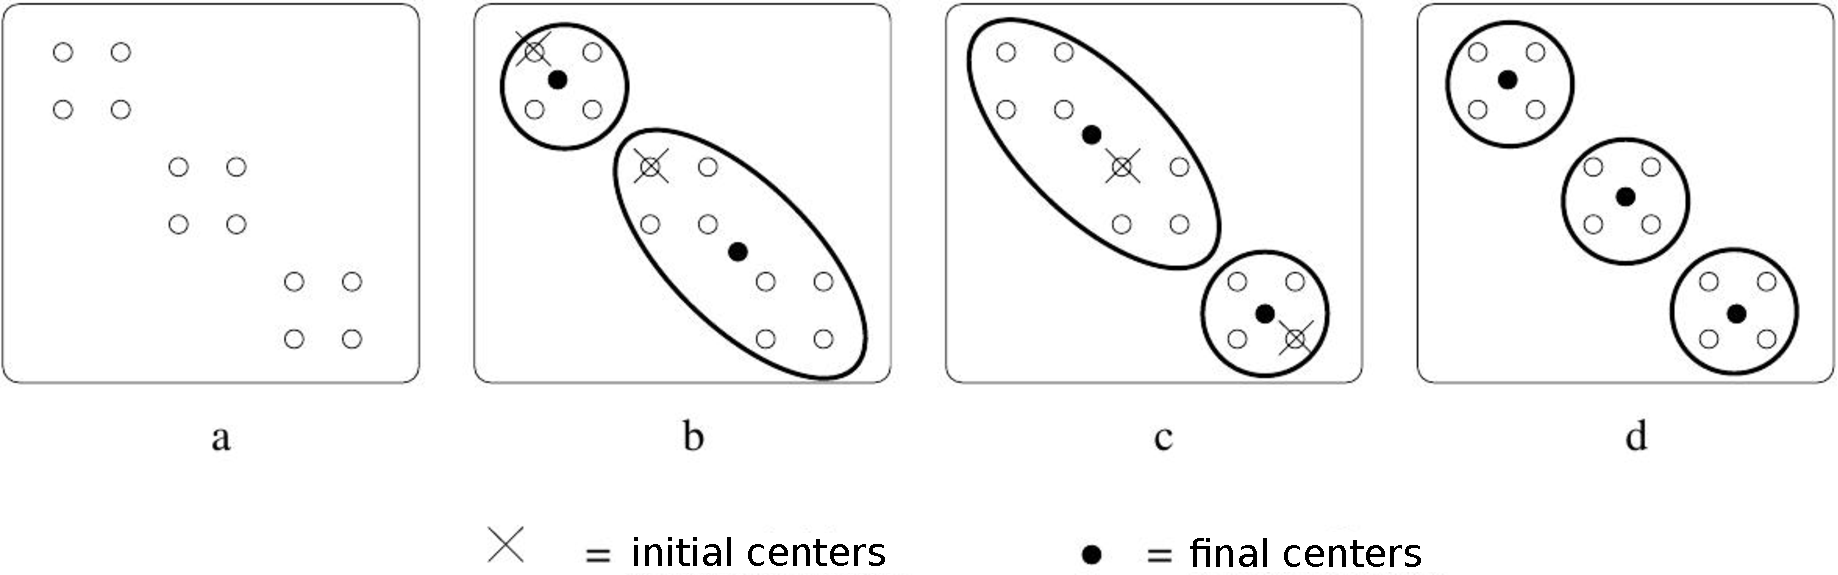
\includegraphics[width=.95\textwidth]{pb_ini_kmeans_en.pdf}\\
    \textcolor{blue}{a) set of points $x_i\in \mathbb{R}^p$ ($p=2$) to classify, b) and c) two clusterings in
      $K=2$ classes with different initial centers, d) clustering in $K=3$ classes.}
    \end{center}


    
    \end{frame}




\begin{frame}
   \frametitle{K-means}
   \begin{block}{Prediction vs Clustering}
   \end{block}
   \begin{minipage}{.49\textwidth}
   \begin{center}
    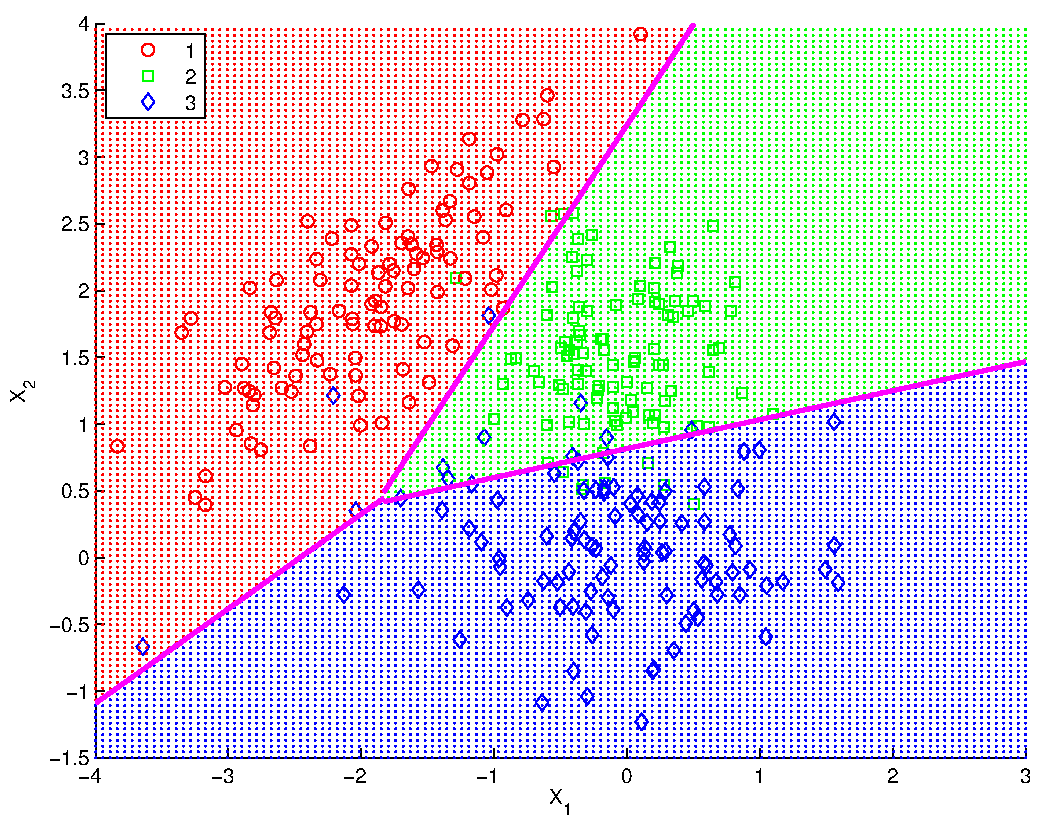
\includegraphics[width=.95\textwidth]{Figs/S02/linear_analysis_bounds.pdf}\\
    \textcolor{blue}{LDA (supervised approach)}
    \end{center}
    \end{minipage} \hfill
    \begin{minipage}{.49\textwidth}
   \begin{center}
    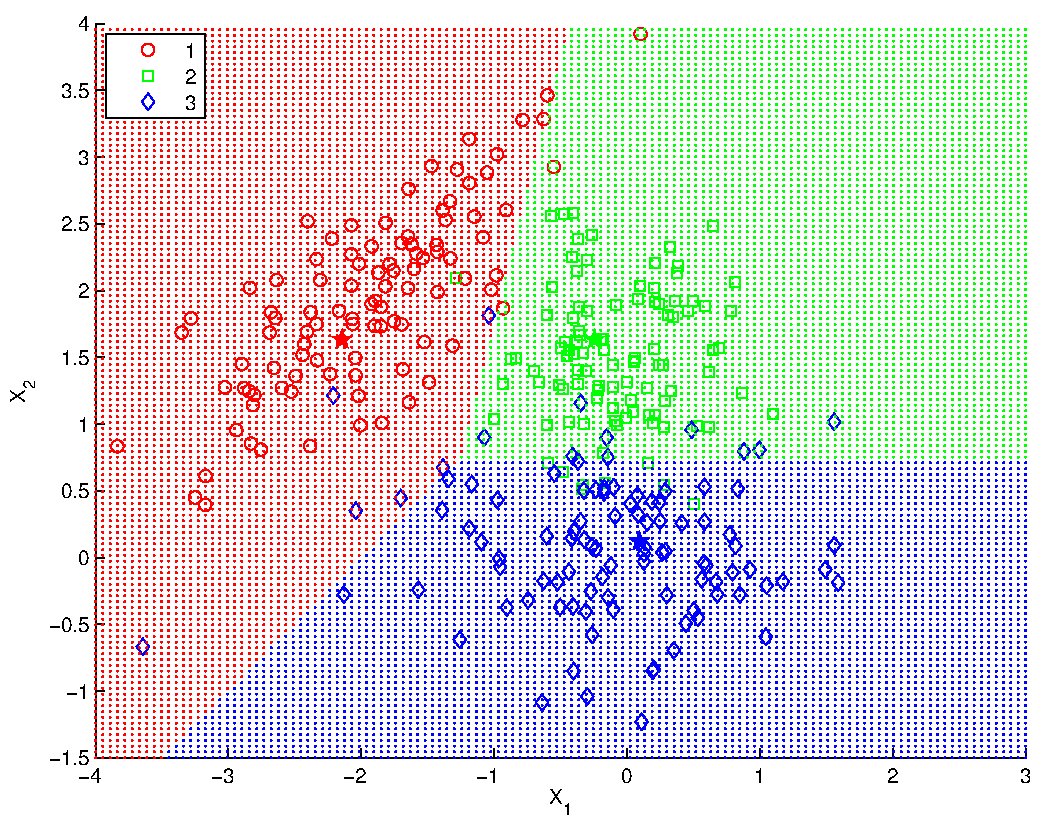
\includegraphics[width=.95\textwidth]{km_bounds.pdf}\\
    \textcolor{blue}{K-means with $K=3$ classes}
    \end{center}
    \end{minipage}
    \begin{itemize}
       \item the points $x_1,\ldots,x_n$ are grouped according to the color of the regions
       \item Prediction: performance on {\em new} data is what matters
       \item Clustering: performance on {\em current} data is what matters
%une nouvelle donnée $x$ est classée dans $\hat{y}$  selon les régions de décision
%       \item K-means~: le centroïde $\mu_{\hat{y}}$ est ensuite mis à jour.
    \end{itemize}
\end{frame}

\section{Model based clustering: EM algorithm}



\begin{frame}{EM (Expectation-Maximization) algorithm}
 

EM method is a general and important tool of statistical analysis:
\begin{itemize}
 \item  method for finding maximum likelihood (ML) or maximum a posteriori (MAP) estimates of parameters in statistical models, by maximizing
 \structuretext{iteratively} the log-likelihood
 \item \structuretext{introduction} of unobserved \structuretext{latent variables $Z$} to decompose the optimization problem in simpler sub-problems in an iterative way
 \item EM iteration \structuretext{alternates} between performing an \structuretext{expectation (E) step}, and a 
 \structuretext{maximization (M) step}
 %where the model depends on unobserved latent variables. The EM iteration alternates between performing an expectation (E) step, which creates a function for the expectation of the log-likelihood evaluated using the current estimate for the parameters, and a maximization (M) step, which computes parameters maximizing the expected log-likelihood found on the E step. These parameter-estimates are then used to determine the distribution of the latent variables in the next E step.
\end{itemize}


\end{frame}


\begin{frame}{EM (Expectation-Maximization) principle}
 
\setbeamertemplate{blocks}[rounded][shadow=true]

\begin{itemize}
 \item $Z$ is a latent variable,
 \item Objective: maximize $\ell(\theta)= \log p(x|\theta)$
\end{itemize}

\begin{block}{Sketch of EM algorithm}
\begin{itemize}
 \item \structuretext{\textbf{E step}}: compute the \structuretext{expectation} of the completed log-likelihood function evaluated using the current estimate for the parameter
 \begin{align*}
  Q\left(\theta,\theta^{(t-1)} \right)&= E_{Z|X,\theta^{(t-1)}} \left[ \log p(x,z|\theta) \right],\\
  &= \int p(z|x,\theta^{(t-1)}) \log{p(x,z|\theta)}dz
 \end{align*}
\item \structuretext{\textbf{M step}}: compute parameters \structuretext{maximizing} the expected log-likelihood
 \begin{align*}
 \theta^{(t)}= \arg \max_{\theta}  Q\left(\theta,\theta^{(t-1)} \right),
 \end{align*}
\item Repeat until convergence of the $\theta^{(t)}$ sequence
\end{itemize}
\end{block}


\end{frame}


\begin{frame}{Application of EM to mixture models: E step}
 
%\setbeamertemplate{blocks}[rounded][shadow=true]
Introducing the latent variables $Y_i$, or equivalently, the binary variables
\begin{align*}
 z_{ik}&= \begin{cases}
          1 & \textrm{if } Y_i=k,\\
          0 & \textrm{otherwise},
         \end{cases}
\end{align*}
the likelihood completed with the r.v. $z_{ik}$ reads
\begin{align*}
 p(x_1,\ldots,x_n,z| \theta)&= \prod_{i=1}^n p(x_i,z|\theta)=\prod_{i=1}^n \prod_{k=1}^K \pi_k \phi(x_i|\theta_k)^{z_{ik}},  
\end{align*}
$$\begin{array}{llcl}
\Rightarrow & \log p(x_1,\ldots,x_n,z| \theta)&=& \sum_{i=1}^n \sum_{k=1}^K z_{ik} 
\log{\left[ \pi_k \phi(x_i|\theta_k) \right]},\medskip\\
\Rightarrow & \structuretext{ Q\left(\theta,\theta^{(t-1)} \right) } & = & \sum_{i=1}^n \sum_{k=1}^K 
\underbrace{E\left[ z_{ik} | x_i, \theta^{(t-1)} \right]}_{\structuretext{t_{ik}^{(t-1)}}} \log{\left( \pi_k \phi(x_i|\theta_k) \right)}
\end{array}$$

where $\begin{array}{lclcl}
\structuretext{t_{ik}^{(t-1)}}&=& \Pr\left(Y_i=k\, \left|\, x_i, \theta^{(t-1)} \right. \right)
&=& 
\structuretext{ 
\frac{  \pi_k^{(t-1)} \phi\left( x_i | \theta^{(t-1)} \right) }
{ \sum_{k=1}^K \pi_k^{(t-1)} \phi\left( x_i | \theta^{(t-1)} \right)   } 
}
\end{array}$



\end{frame}


\begin{frame}{Gaussian mixture models: M step}

Find $\theta\equiv\theta^{(t)}$ maximizing 
$Q\left(\theta,\theta^{(t-1)} \right) = \sum_{i=1}^n \sum_{k=1}^K t_{ik}^{(t-1)} \log{\left[ \pi_k \phi(x_i|\theta_k) \right]}$

\begin{itemize}
%  \item Find $\theta=\theta^{(t)}$ maximizing 
%$$Q\left(\theta,\theta^{(t-1)} \right) = \sum_{i=1}^n \sum_{k=1}^K t_{ik}^{(t-1)} \log{\left[ \pi_k \phi(x_i|\theta_k) \right]}$$
  \item For any mixture model (i.e. $\forall \phi$): \vspace{-2mm}
  $$
   \structuretext{ \pi_k^{(t)} }= \frac{1}{n} \sum_{i=1}^n \theta^{(t-1)}
  $$\vspace{-4mm}\\
  \item For a Gaussian mixture model $\theta=\{\mu_k,\Sigma_k\}$ and 
  \begin{align*}
   \structuretext{ \mu_k^{(t)} } &= \frac{ \sum_{i=1}^n t_{ik}^{(t-1)} x_i }{\sum_{i=1}^n t_{ik}^{(t-1)}},\\
   \structuretext{ \Sigma_k^{(t)} } &= \frac{ \sum_{i=1}^n t_{ik}^{(t-1)} \left( x_i -\mu_k^{(t)} \right) \left( x_i -\mu_k^{(t)} \right)^T }
   {\sum_{i=1}^n t_{ik}^{(t-1)}},
  \end{align*}
  \item empirical averages weighted by the posterior probability in $\theta^{(t-1)}$,  $t_{ik}^{(t-1)} \equiv \Pr{\left(Y_i=k\,|\, x_i,\theta^{(t-1)} \right) }$ 
  \item[\doigt] \structuretext{soft-thresholding} algorithm
 \end{itemize}




\end{frame}



\begin{frame}{EM algorithm for Gaussian mixture models}
\setbeamertemplate{blocks}[rounded][shadow=true]

\begin{block}{EM clustering}
\begin{itemize}
\item Initialize $\pi_k^{(0)}$, $\mu_k^{(0)}$,  $\Sigma_k^{(0)}$, for $k=1,\ldots,K$
\item For $t=1,\ldots$ until convergence
\begin{itemize}
\item[\structuretext{\textbf{(E)}}] for $i=1,\ldots,n$, $k=1,\ldots,K$,
compute $t_{ik}^{(t-1)} \equiv \Pr{\left(Y_i=k\,|\, x_i,\theta^{(t-1)} \right) }$
\item[\structuretext{\textbf{(M)}}] for $k=1,\ldots,K$, compute $\pi_k^{(t)}$, $\mu_k^{(t)}$,  $\Sigma_k^{(t)}$
 \end{itemize}
  \end{itemize}
\end{block}

\setbeamertemplate{blocks}[rounded][shadow=false]

\begin{block}{Prediction/Correction structure}
 \begin{itemize}
 \item E step $\Leftrightarrow$ prediction step
 \item M step $\Leftrightarrow$ update/correction step
\end{itemize}
\end{block}


\begin{block}{Convergence}
 \begin{itemize}
 \item EM: convergence toward a local maximum of the log-likelihood
 \item[\doigtr] no guaranty of convergence toward the optimal solution (depend on the initial values).. 
\end{itemize}
\end{block}


\end{frame}


\begin{frame}
   \frametitle{Gaussian mixture model and EM algorithm}
   \begin{block}{Prediction vs Clustering}
   \end{block}
   \begin{minipage}{.49\textwidth}
   \begin{center}
    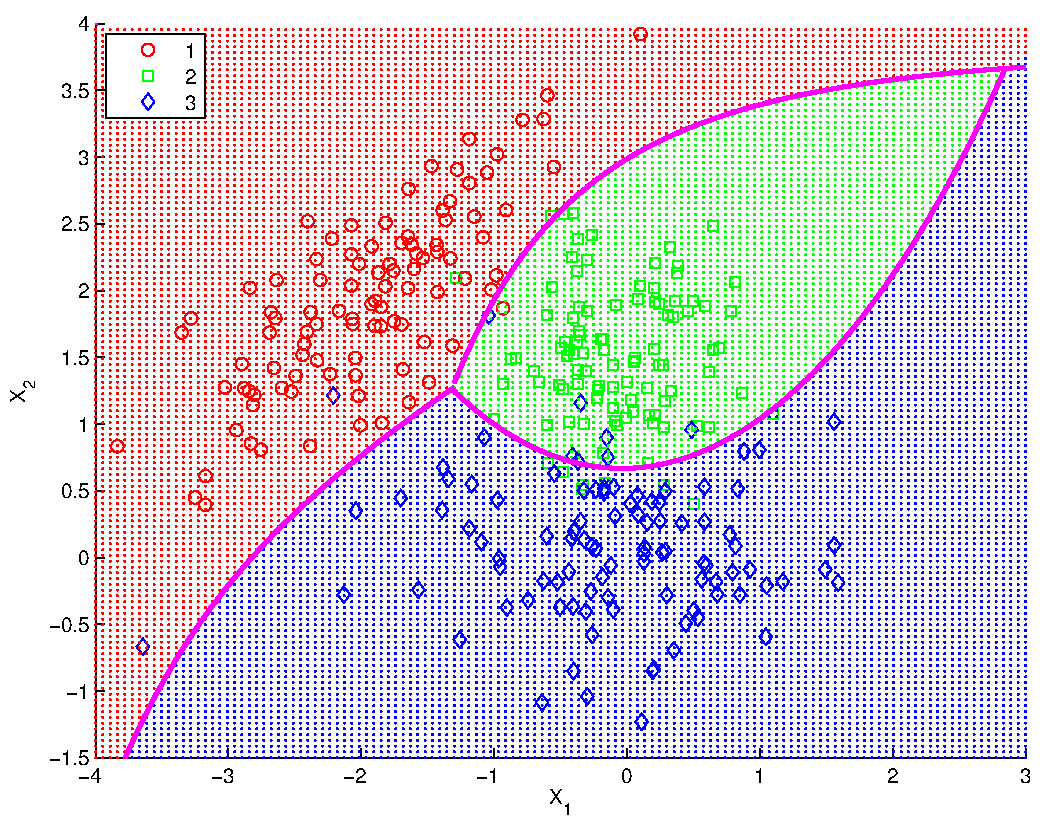
\includegraphics[width=.95\textwidth]{Figs/S02/quad_analysis_bounds.pdf}\\
    \textcolor{blue}{QDA  (supervised approach)}
    \end{center}
    \end{minipage} \hfill
    \begin{minipage}{.49\textwidth}
   \begin{center}
    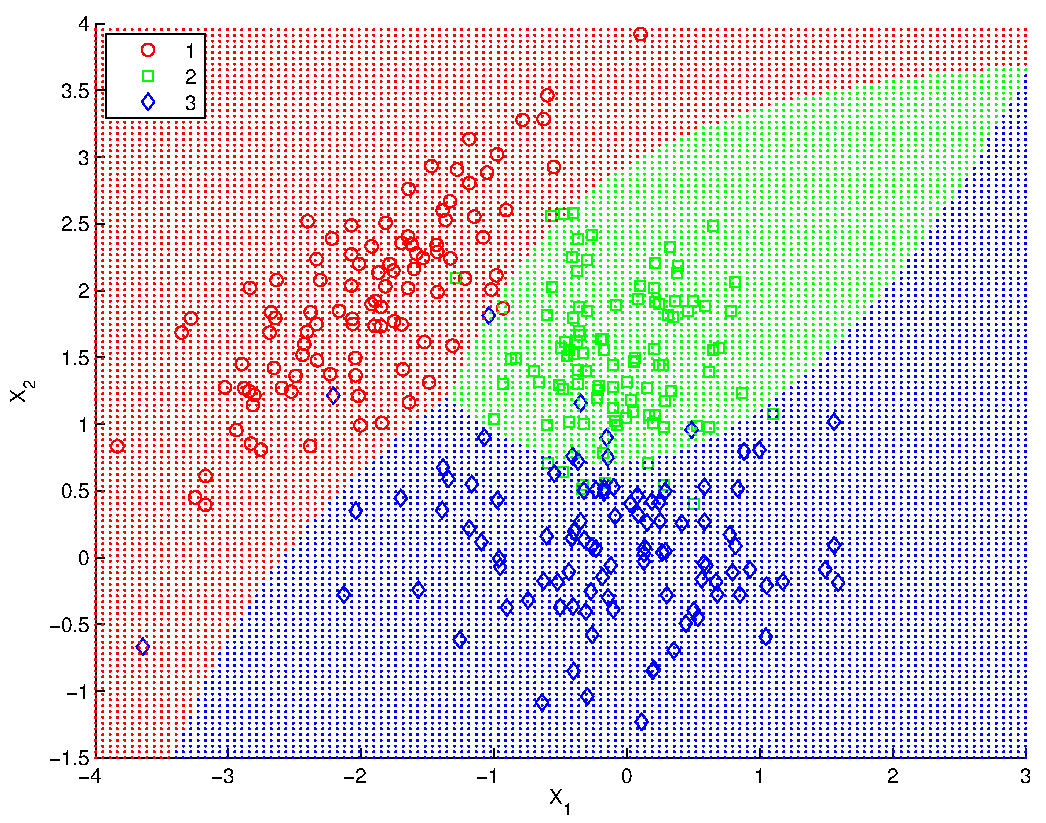
\includegraphics[width=.95\textwidth]{gm_bounds.pdf}\\
    \textcolor{blue}{EM with $K=3$ classes}
    \end{center}
    \end{minipage}
    %\begin{itemize}
    %   \item les données $x_1,\ldots,x_n$ sont classées dans la classe $\hat{y}_i$ selon les régions de décision (couleurs identiques à celles des classes)
    %   \item une nouvelle donnée $x$ est classée  dans $\hat{y}$  selon les régions de décision
    %   \item EM~: le centroïde ($\mu_{\hat{y}}, \Sigma_{\hat{y}})$ et les probas
    %   $\pi_1,\ldots,\pi_K$ sont ensuite mis à jour
    %\end{itemize}
    \begin{itemize}
       \item the points $x_1,\ldots,x_n$ are grouped according to the color of the regions
       \item Prediction: performance on {\em new} data is what matters
       \item Clustering: performance on {\em current} data is what matters
    \end{itemize}
\end{frame}

\begin{frame}
   \frametitle{Gaussian mixture model and EM algorithm}
   \begin{block}{Estimation of the mixture density $f$}
   \end{block}
   \begin{minipage}{.49\textwidth}
   \begin{center}
    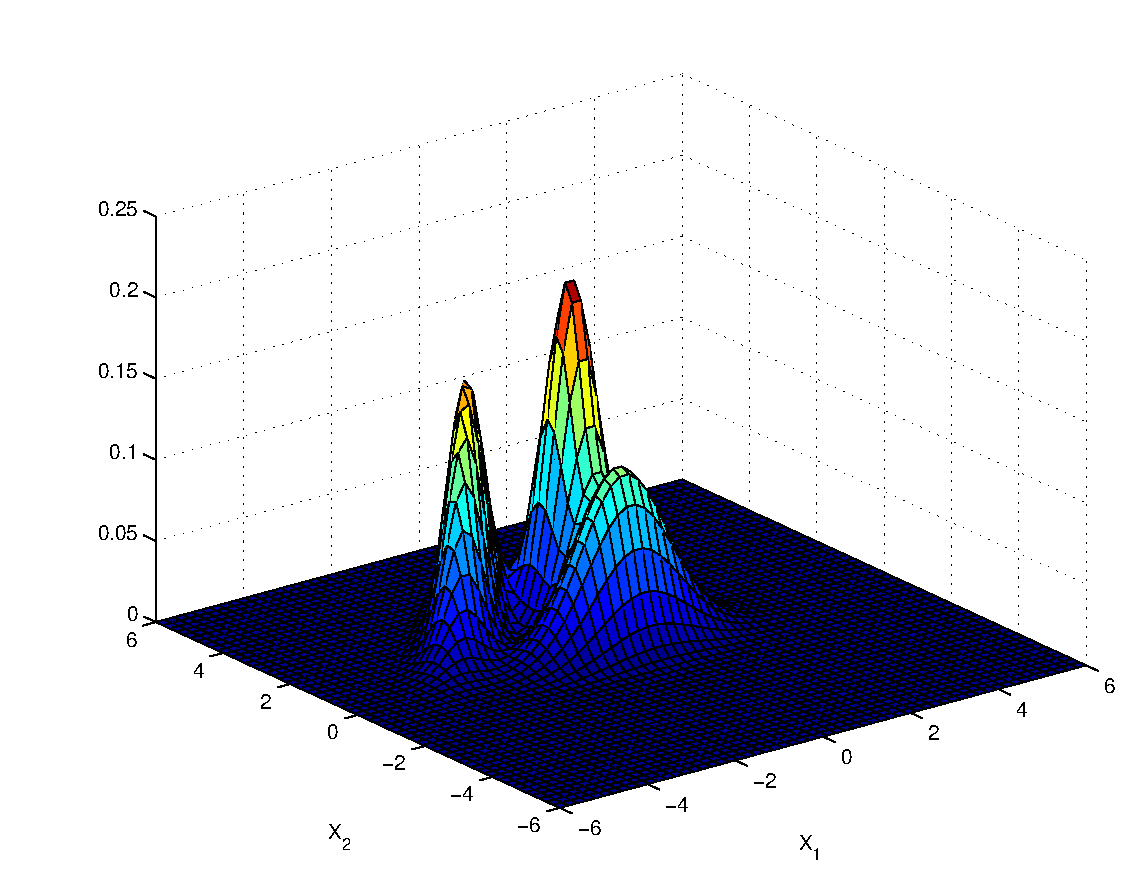
\includegraphics[width=.95\textwidth]{pdf_gmth_3d.pdf}\\
    \textcolor{blue}{True density of the data points $x_1,\ldots,x_n$}
    \end{center}
    \end{minipage} \hfill
    \begin{minipage}{.49\textwidth}
   \begin{center}
    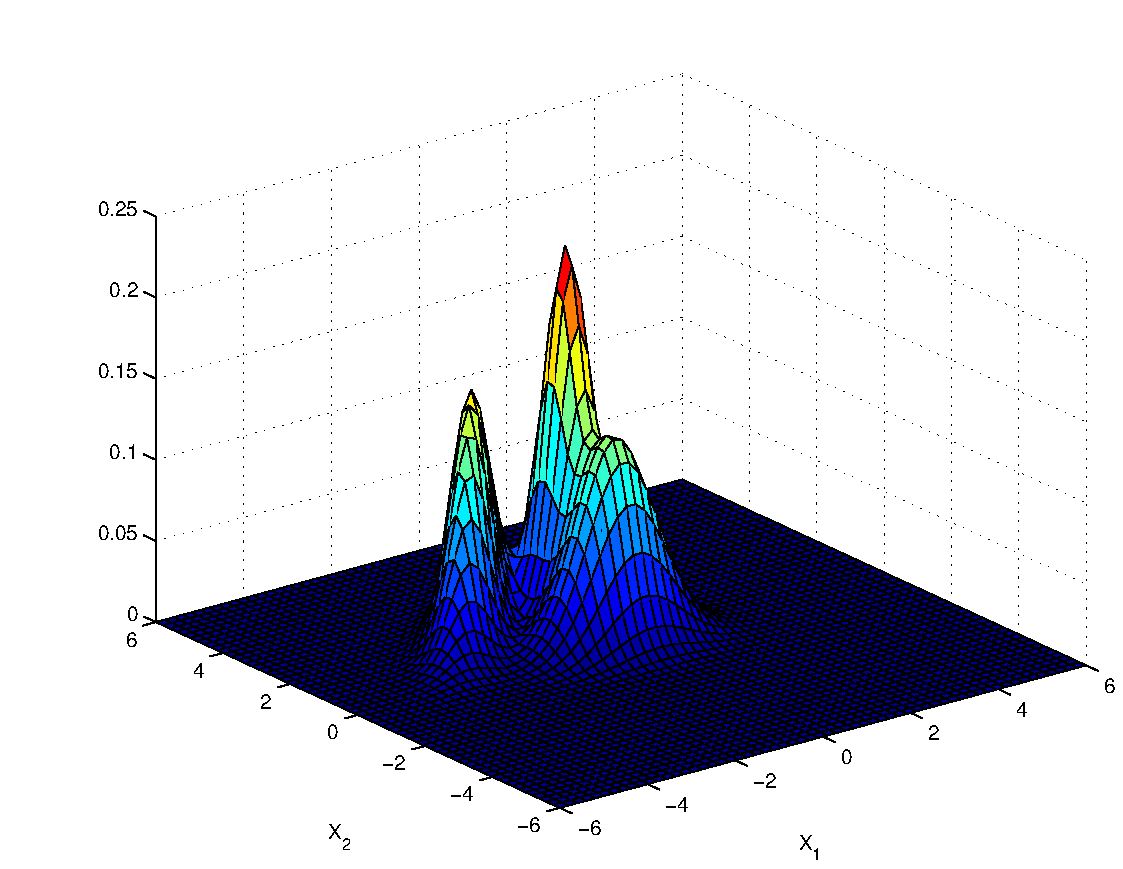
\includegraphics[width=.95\textwidth]{pdf_gmfit_3d.pdf}\\
    \textcolor{blue}{Estimated density with EM ($K=3$ classes)}
    \end{center}
    \end{minipage}
\end{frame}

\section{Comparison K-means vs Algo EM}

\begin{frame}
   \frametitle{Comparison K-means vs Algo EM}

   \begin{block}{$2$ classes with overlapping and very different dispersions (covariances $\Sigma_k$) }
   \end{block}

\begin{minipage}{.49\textwidth}
\begin{center}
    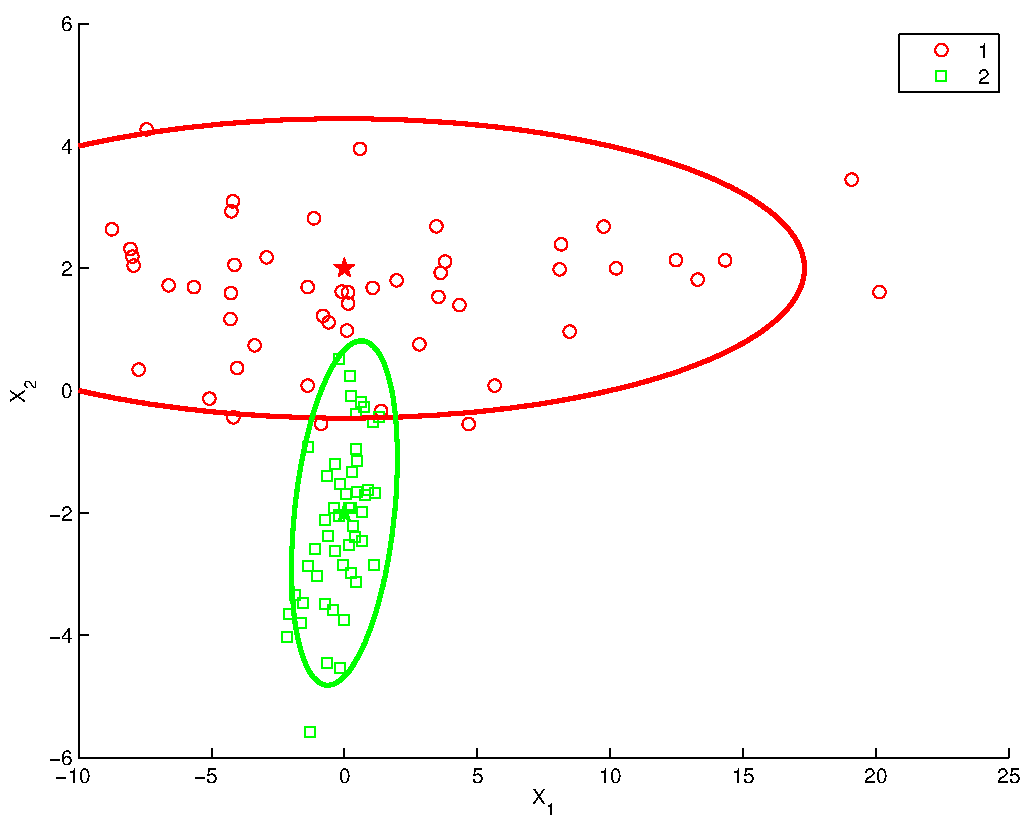
\includegraphics[width=\textwidth]{GMvsKM.pdf}\\
    \textcolor{blue}{Data $x_1,\ldots,x_n$, classes and true $95$\% confidence regions}
\end{center}
\end{minipage}
\hfill
\begin{minipage}{.49\textwidth}
\begin{center}
    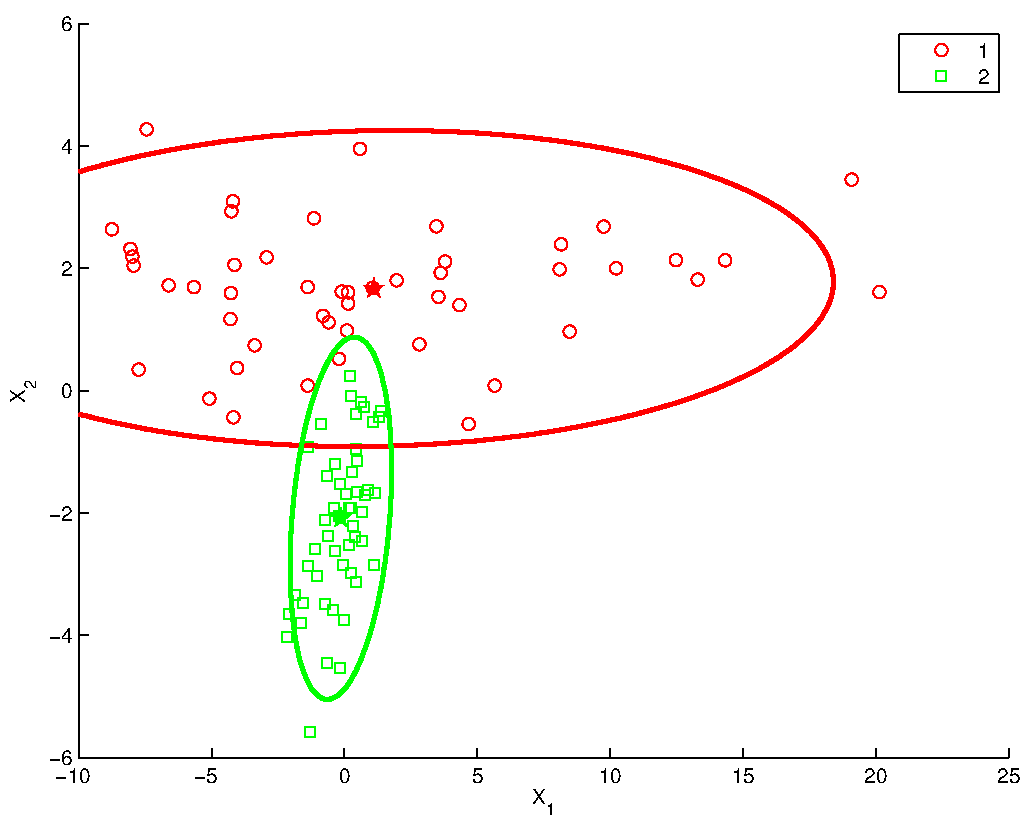
\includegraphics[width=\textwidth]{GMvsKM_gm.pdf}\\
    \textcolor{blue}{Clustering with EM ($K=2$) and estimated $95$\% confidence regions}
\end{center}
\end{minipage}

\end{frame}

\begin{frame}
   \frametitle{Comparison K-means vs Algo EM}

\begin{block}{$2$ classes with overlapping and very different dispersions (covariances $\Sigma_k$) }
   \end{block}
   
\begin{minipage}{.49\textwidth}
\begin{center}
    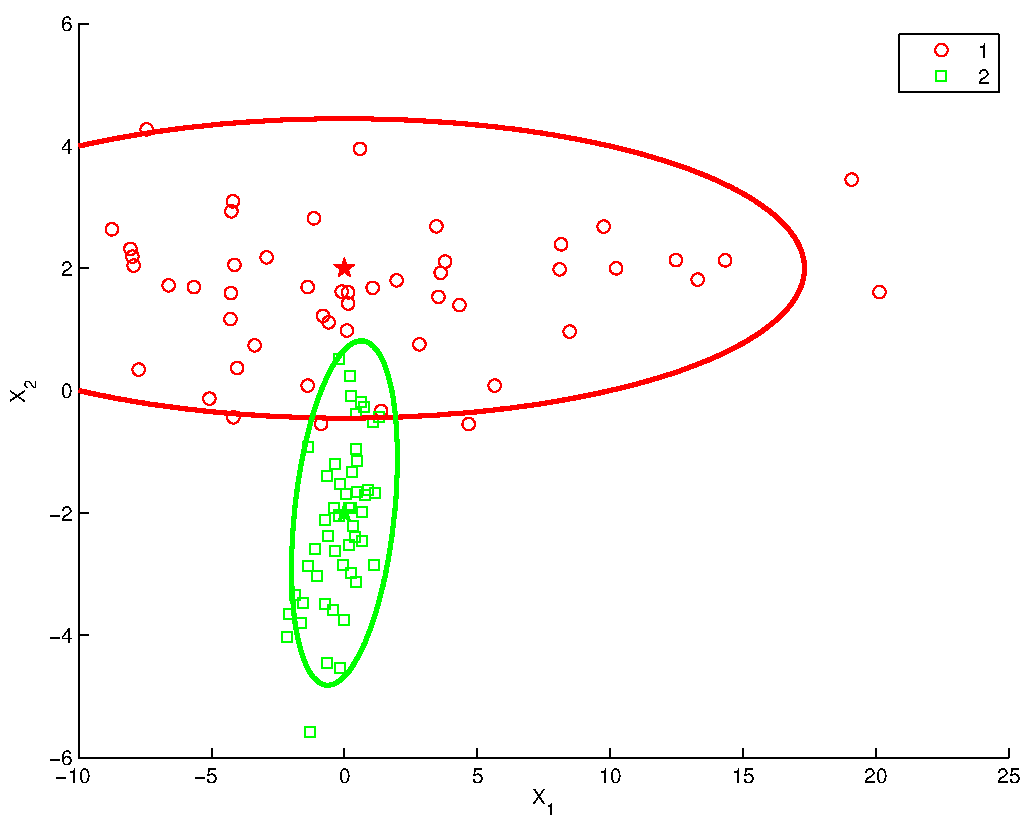
\includegraphics[width=\textwidth]{GMvsKM.pdf}\\
    \textcolor{blue}{Data $x_1,\ldots,x_n$, classes and true $95$\% confidence regions}
\end{center}
\end{minipage}
\hfill
\begin{minipage}{.49\textwidth}
\begin{center}
    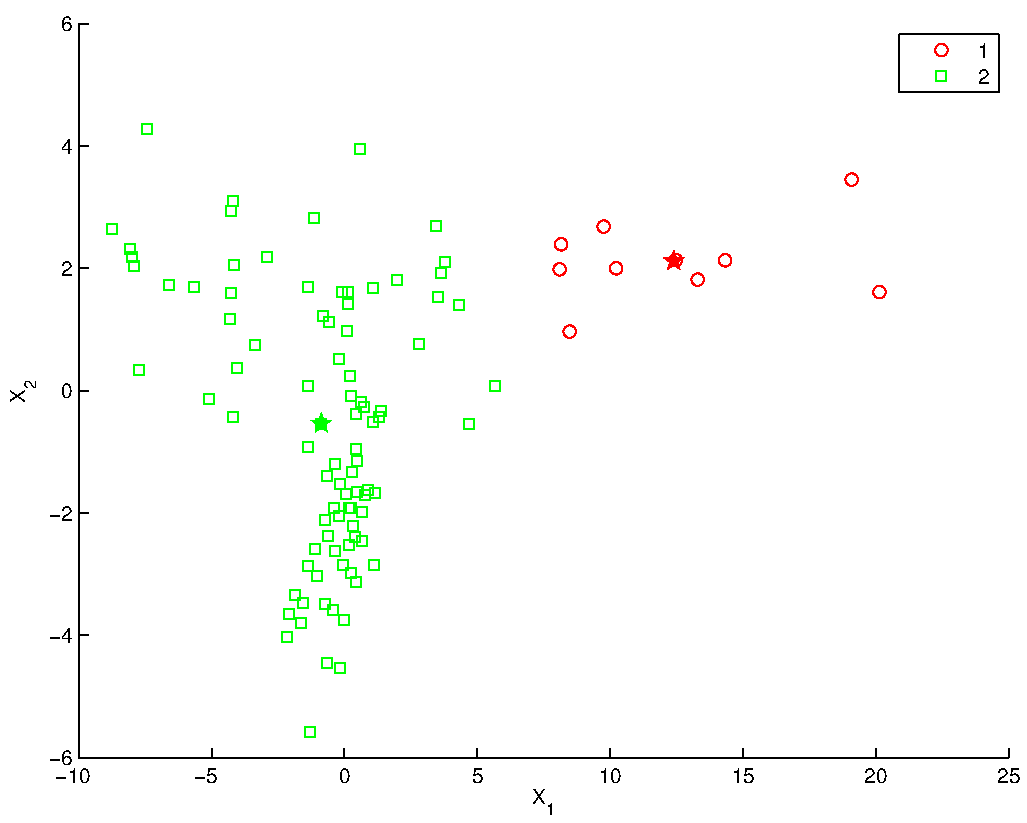
\includegraphics[width=\textwidth]{GMvsKM_km.pdf}\\
    \textcolor{blue}{Classification with K-means\\ ($K=2$)}
\end{center}
\end{minipage}

\end{frame}


\section{Model selection}



\begin{frame}
   \frametitle{Model selection: estimation of $K$}

   \begin{block}{Minimization of a penalized log-likelihood criterion}
%\vspace{-5mm}
   \begin{align*} C(K)&= -\hat{l}(x ; K) + \textrm{pen}(K,n)
   \end{align*}
 %  \vspace{-5mm}
   \begin{itemize}
    \item $\hat{l}(x; K) \equiv l(x ; \hat{\theta}_K, K)$ with $\hat{\theta}_K$ the MLE
    of the model parameters with $K$ classes (profile log-likelihood  w.r.t $K$)
   \end{itemize}
   
  Trade-off between two terms to minimize
   \begin{itemize}
    \item $-\hat{l}(x ; K)$~: fidelity to the data (likelihood)
    \item $\textrm{pen}(K,n)$~: low complexity of the model
   \end{itemize}
   \end{block}

 
\end{frame}

\begin{frame}
   \frametitle{Model selection: BIC criterion}

  \begin{block}{Bayesian Information Criterion (BIC)}
   Asymptotic ($n \gg m_K$)  criterion for Bayesian models (i.e. with a prior on the model parameters)
   $$ \textrm{pen}(K,n)=\frac{1}{2} m_K \log(n)$$
   
   \begin{itemize}
    \item $n$ is the size of the data
    \item $m_K$ is the effective number of parameters for the $K$ class model
    \end{itemize}
   Equivalent to minimize the following criterion
   \begin{align*}
    \structuretext{\textrm{BIC}(K)} & = \structuretext{-2 \hat{l}(x ; K) + m_K \log(n) } 
    \end{align*}
   \end{block}


\end{frame}


\begin{frame}
   \frametitle{Model selection: estimation of $K$}

   \begin{block}{Example of synthetic data generated according to
   a mixture of $K=3$ Gaussians}
   \end{block}

\begin{minipage}{.49\textwidth}
\begin{center}
    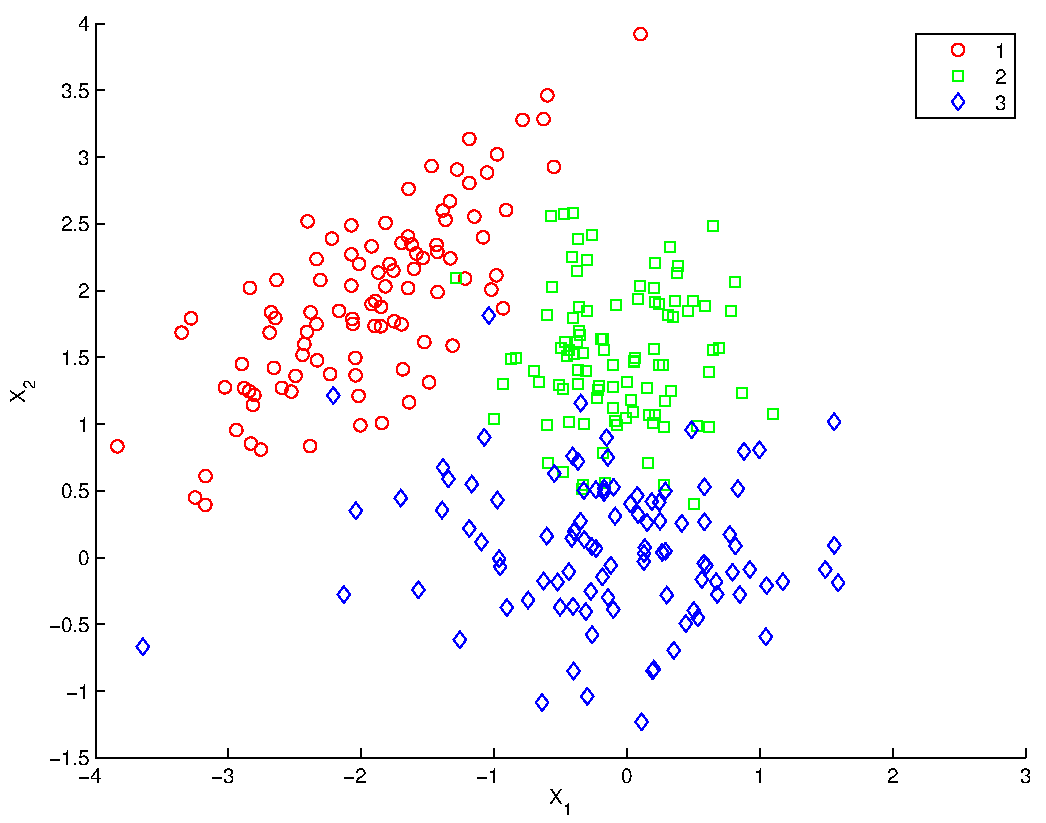
\includegraphics[width=\textwidth]{Figs/S02/discr_analysis_ex.pdf}\\
    \textcolor{blue}{Dataset $x_1,\ldots,x_n$ ($n=500$ realizations)}
\end{center}
\end{minipage}
\hfill
\begin{minipage}{.49\textwidth}
\begin{center}
    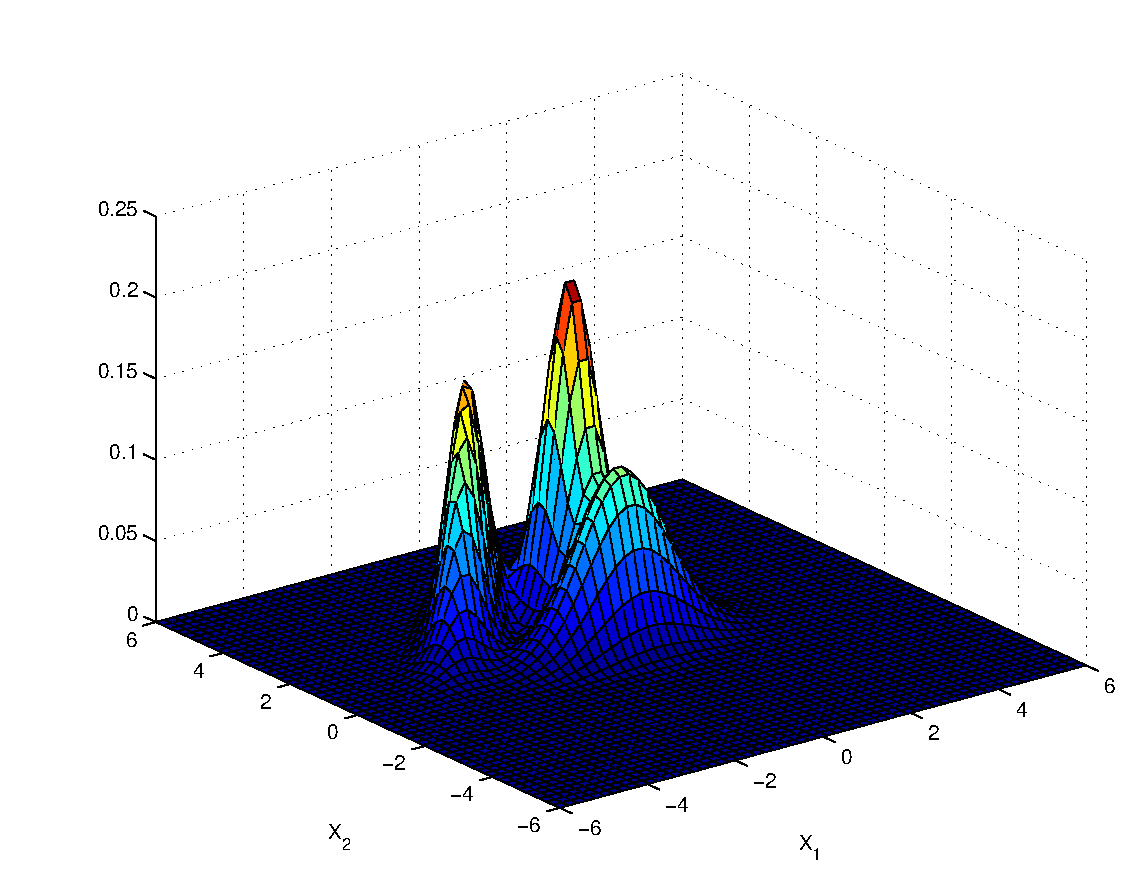
\includegraphics[width=\textwidth]{pdf_gmth_3d.pdf}\\
    \textcolor{blue}{True density $f$}
\end{center}
\end{minipage}
\end{frame}


\begin{frame}
   \frametitle{Model selection: estimation of $K$}
   \vspace{3mm}
{\small
    Gaussian mixture:
    $
      m_K=   \underbrace{K-1}_{\pi_1,\ldots,\pi_{K-1}}  + \  K \times  \underbrace{p}_{\mu_k}  + \  K  \times \underbrace{\frac{p(p+1)}{2}}_{\Sigma_k}
    $
    }   \vspace{-3mm}
   \begin{block}{BIC criterion w.r.t. $K$}
   \end{block}
\begin{center}
    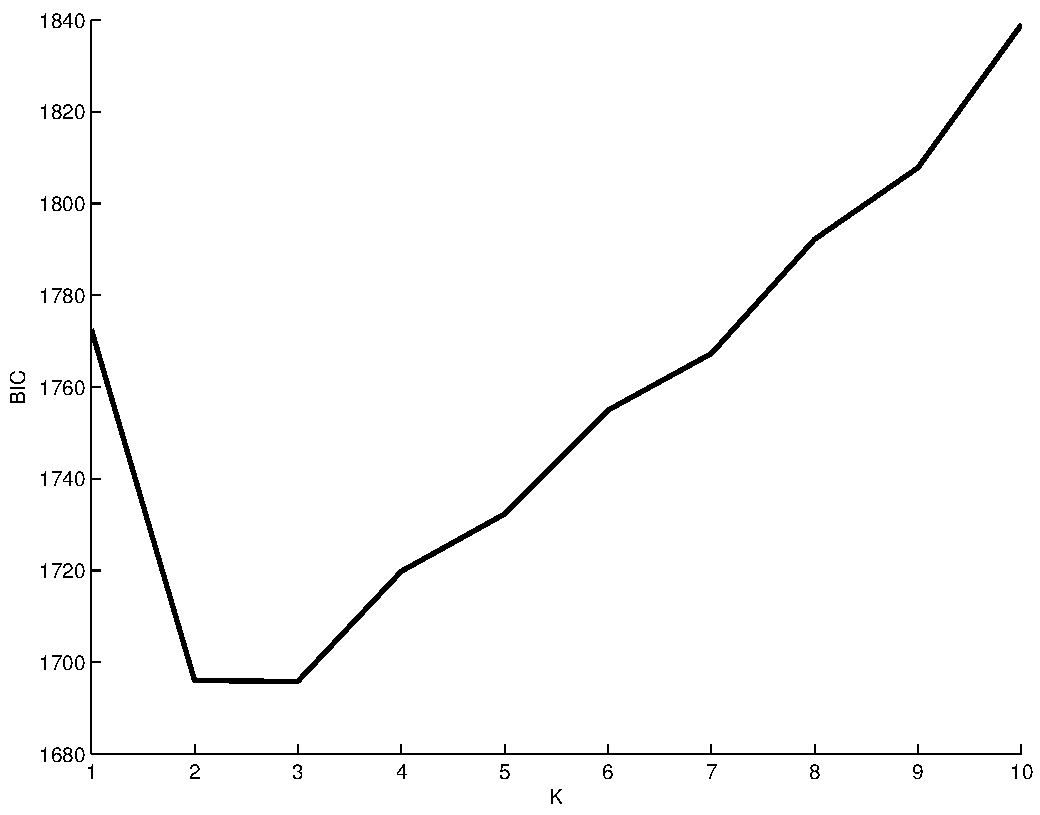
\includegraphics[width=.5\textwidth]{BICvsK.pdf}\\
\end{center}
\begin{itemize}
   \item[$\Rightarrow$] $\hat{K}=2$ or $\hat{K}=3$ (true value $K=3$)
\end{itemize}

\end{frame}

\end{document}
